\section{Basic User Interface Overview}
\subsection{Main Window Layout}
All user interaction takes place within the main window.  There are several components to this window -- the most obvious of which is the \ui{3D view}, which allows you to interact with a three-dimensional projection of the core, assembly, pin, or duct you're working with.  To the left of the 3D view are the \ui{input}[input panel] and the \ui{properties panel}s.  Above the input panel is the \ui{toolbar}, which has icons for often used actions.  Above the toolbar is the \ui{menu}. Refer to Figure \ref{fig:mainwindow1} to see these pictorally.

\begin{figure}[H]
	\begin{center}
		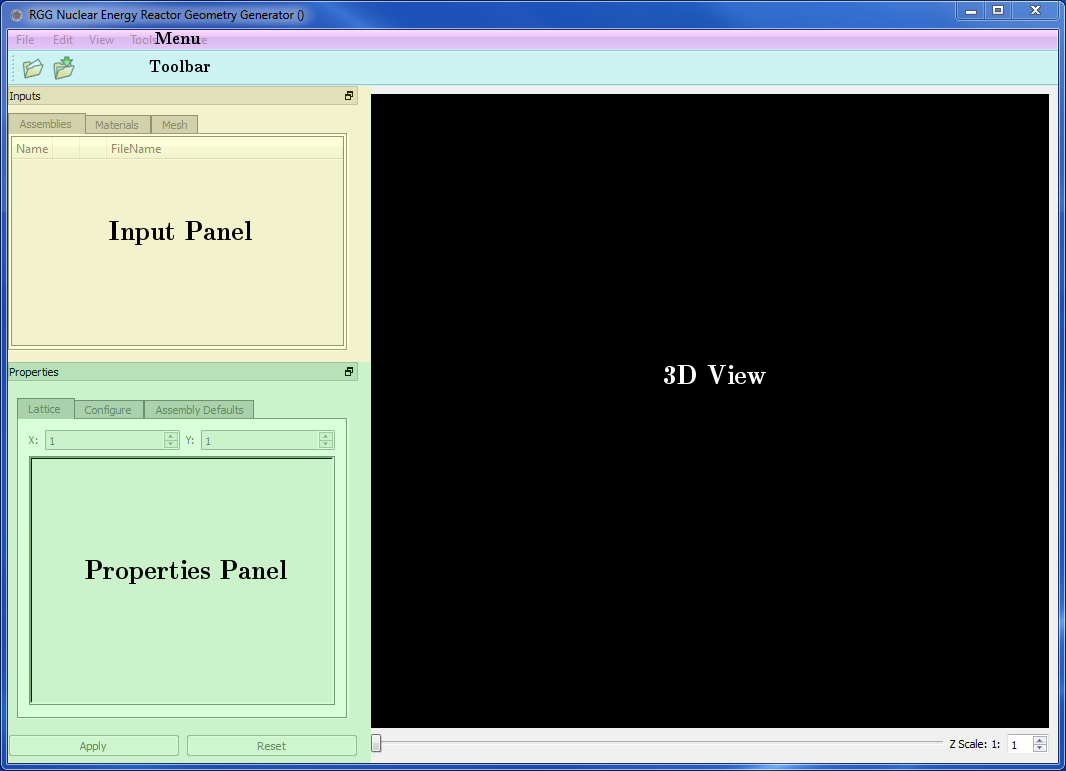
\includegraphics[width=\linewidth]{Images/main-window-layout.png}
		\caption{Layout of the \ui{main window}.}
		\label{fig:mainwindow1}
	\end{center}
\end{figure}


\subsection{Input Panel}
The \ui{input panel} has three tabs: the \ui{assemblies tab}, the \ui{materials tab}, and the \ui{mesh tab}.

\subsubsection{Assemblies Tab}
The \ui{assemblies tab} shows the hierarchal nature of the core, assemblies, pins and ducts.  Recall that a core is composed of assemblies which are placed in the core's lattice, and that these assemblies are in turn composed of pins and ducts that are placed in the assembly lattice.

\begin{figure}[H]
	\begin{center}
		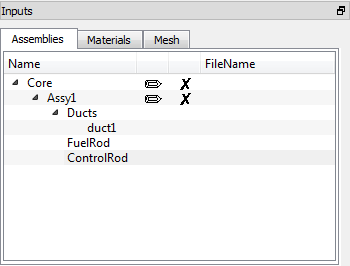
\includegraphics[width=0.5\linewidth]{Images/assemblies-tab.png}
		\caption{The assemblies tab shows the core, assembly, pin, and duct hierarchy.}
		\label{fig:mainwindow2}
	\end{center}
\end{figure}

Note you can check to see if the core or an assembly has had changes made to it since the last save.  A \ui{pencil icon} (as above in Figure \ref{fig:mainwindow2}) indicates that edits have been made since the file was last saved.  A \ui{green box icon} indicates that the file is up to date.

You can also see the status of mesh files here.  An \ui{x icon} (as above, to the right of the \ui{pencil icon}) indicates that mesh files have not been generated (or haven't been recreated since edits to the associated core or assembly), while \ui{green box icons} indicate that they are up to date.

\subsubsection{Materials Tab}
\toIndex{Materials}
The \ui{materials tab} details the list of available materials, their associated colors, and whether or not they are viewable.  You can use this tab to create, remove, import, and export materials, as well as edit the labels and colors of materials and toggle whether or not they are shown in the 3D view.

\begin{figure}[h]
	\begin{center}
		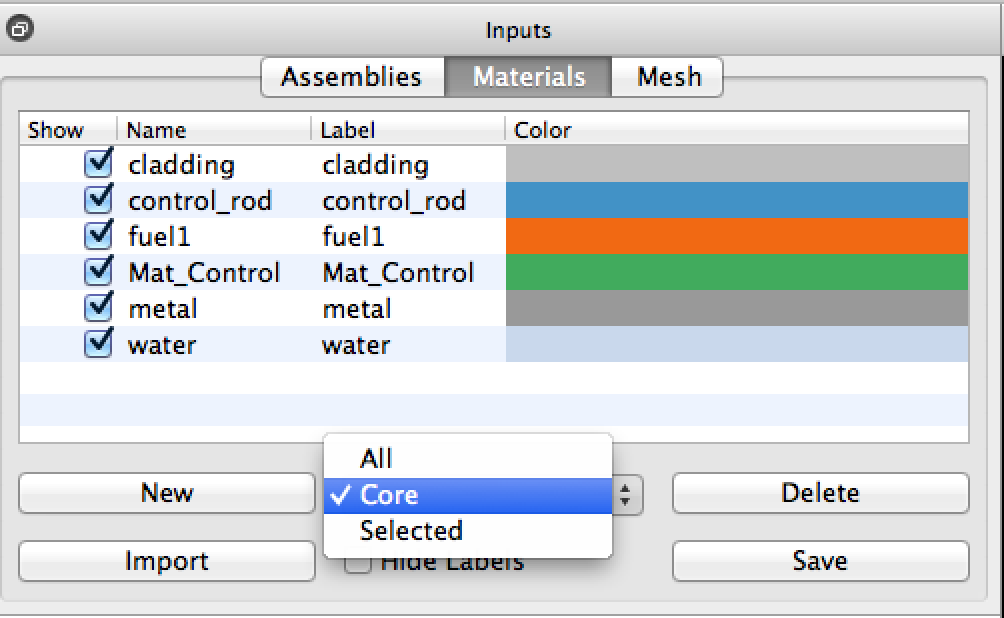
\includegraphics[width=0.5\linewidth]{Images/materials-tab.png}
		\caption{The materials tab shows available materials.}
		\label{fig:mainwindow3}
	\end{center}
\end{figure}

\subsubsection{Mesh Tab}
The \ui{mesh tab} allows you to control the viewing of the mesh.  It has the options to control what shows up in the \ui{3D mesh view}, including the ability to show volumes, boundaries, surfaces, Neumann sets, Dirichlet sets, Material sets, show mesh edges, and to colorize the different volumes.  More information on this tab is given in Section \ref{section:DisplayingMeshes}.

\subsection{Properties Panel}
The \ui{properties panel} changes depending on the current state of the input panel's \ui{assemblies tab}.

\begin{itemize}
	\item{If you're clicking on a core, it will display three tabs: the \ui{lattice tab}, the \ui{configure tab}, and the \ui{assembly defaults tab}.}
	\item{If you're clicking on an assembly, it will display the \ui{lattice tab} and \ui{configure tab}, and the \ui{defaults tab} (not to be confused with the assembly defaults tab).  Note that the assembly has a different \ui{latticeSe tab} and \ui{configure tab} from the core.}
	\item{If you're clicking on a duct, it will display the \ui{duct tab}.}
	\item{If you're clicking on a pin, it will display the \ui{pin tab}.}
\end{itemize}

\begin{commonerrors}
	The \ui{assembly defaults tab} controls global settings for assemblies.  As such, it's displayed when clicking on the core in the \ui{assemblies tab}.  The \ui{defaults tab} controls settings on a per-assembly basis; it's found when clicking on an assembly in the \ui{assemblies tab}.
\end{commonerrors}

\subsubsection{Lattice Tab}
The \ui{lattice tab} illustrates the placement of assemblies of the core (if this is the core lattice -- you're clicking on the core in the \ui{assemblies tab}) or the placement of pins (if this is an assembly lattice -- you're clicking on an assembly in the \ui{assemblies tab}).  See Figure \ref{fig:latticetab}.

Each assembly or pin represented here will be filled with its corresponding key color.

You can edit this information by specifying the number of layers (in a hexagonal core) or the dimensions (in a rectilinear core) to get the desired lattice geometry, and then right-click on each cell to select the desired assembly or pin.  Alternatively, you can drag and drop an existing component onto the cell.

This tab is also where the key color for this component is specifed.

\begin{figure}[h]
	\begin{center}
		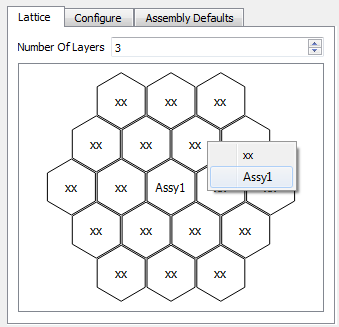
\includegraphics[width=0.3\linewidth]{Images/hex-19.png}
		\caption{The lattice tab for a three-layer full hexagonal core.  The user has right clicked to place an assembly.}
		\label{fig:latticetab}
	\end{center}
\end{figure}

\subsubsection{Configure Tab}
This tab allows you to customize other meshing parameters from MeshKit files which are not currently provided an interface in the GUI. See Chapter \ref{chapter:Meshing} for information on how to mesh your core.

When building a full hexagonal core, $\frac{1}{6}$ flat hexagonal core, or a $\frac{1}{12}$ hexagonal core you should include a rotation of $30^\circ$ in each assembly to prevent assemblies from overlapping each other, as shown in \ref{fig:configuretab}.  See more on this in Section \ref{section:RotateAssembly30}.

\begin{figure}[h]
	\begin{center}
		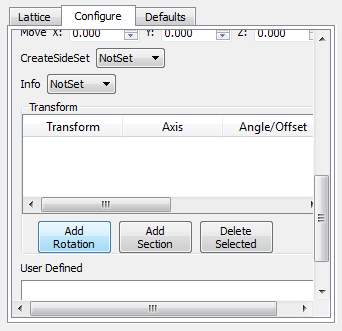
\includegraphics[width=0.4\linewidth]{Images/hex-16.png}
		\caption{Adding a $30^\circ$ rotation in the configure tab of an assembly.}
		\label{fig:configuretab}
	\end{center}
\end{figure}

\subsubsection{Assembly Defaults Tab}
The \ui{assembly defaults tab} allows you to specify general meshing information.  You can set whether the mesh you want to generate will be tetrahedral or hexahedral, and also change the default dimensions of the ducts comprising your core.  Changing these values will propagate all the way down to every component, so you can change it all in one place instead of adjusting the height of every duct in every assembly.

\subsubsection{Defaults Tab}
The \ui{defaults tab} allows you to configure the pitch of the assembly.  You can either specify it manually or calculate it using the \ui{calculate button}.

\subsubsection{Duct Tab}
The \ui{duct tab} exposes the different configuration options for a duct piece.  You can change the position and dimensional settings towards the top, the duct pitch, and the duct material (with associated normalized thickness, if desired).

\subsubsection{Pin Tab}
The \ui{pin tab} allows you to change the key color of the pin, specify the pin material(s), and create, remove, or edit pin pieces.

\begin{figure}[h]
	\begin{center}
		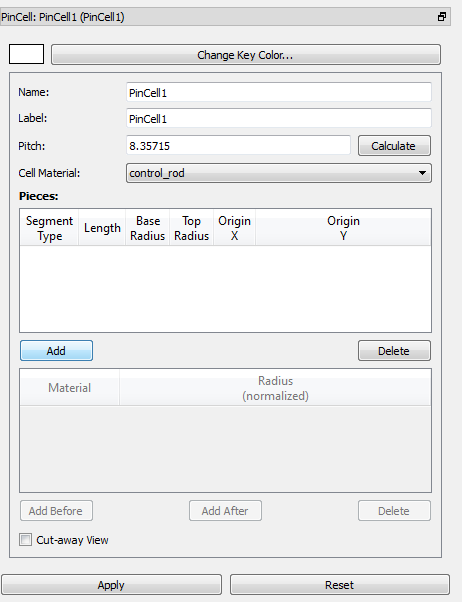
\includegraphics[width=0.4\linewidth]{Images/hex-11.png}
		\caption{The pin tab.}
		\label{fig:pintab}
	\end{center}
\end{figure}

\subsection{3D View}
The \ui{3D view} displays a representation of the current component.  You can use the following controls to interact with it:

\begin{itemize}
	\item{To rotate, click with the left mouse button.}
	\item{To pan, either shift-click with the left mouse button or use the middle mouse button.}
	\item{To zoom, click with the right mouse button.}
\end{itemize}

Similar to the \ui{properties panel}, the \ui{3D view} changes depending on what is selected in the assemblies tab of the input panel.

\begin{itemize}
	\item{If you're clicking on a core, it will display the entire core.}
	\item{If you're clicking on an assembly or a duct, it will display the assembly.}
	\item{If you're clicking on a pin, it will display the pin.}
\end{itemize}